\section{Background}

In this chapter, a short overview will over the current state of the art for visualization inside the field of scientific computing is given. The chapter will start out with a first look at Julia.

\subsection{Related Work}

\subsubsection{The Julia Programming Language}

Bringing Julia's ease of use and speed to a dynamic visualization library is one of the main goals.
So Julia plays a crucial role in this thesis. 
It is the most important previous work, as much as Julia is the main used technology.
This chapter gives a short introduction to the Julia Programming Language.

Julia was published in 2012 which makes it a very new language. It is currently at version 0.3.7 for stable and 0.4 development.
Following common versioning conventions this means Julia is still in an early release phase with the core features and names suspicable to change.
Julia is a multi-paradigma language for scientific computing and it is using the compiler infrastructure \ac{LLVM} to generate fast assembly code.

Some of its most important features are multiple dispatch, a dynamic type system, macros, good performance and an interface to C/C++ and Python.
The focus on scientific computing means that Julia's standard library is equipped with a lot of functions, data structures and specialized syntax for implementing complex math.
It promises to approach C speed while being a dynamic language which is easy to use.
This is made possible by the compile process which can be described as statically compiled at run-time, which is known as \ac{JIT} compilation.
Julia uses a garbage collector, taking the task of memory management away from the programmer.
There are quite a few things Julia promises to the developer which includes the following items\cite{WhyJulia}:

\begin{itemize}
	\item C-like performance
	\item native C interface
	\item macros similar to Lisp
	\item mathematical notations like Matlab
	\item as good at general purpose programming as Python
	\item easy for statistics as R.
\end{itemize}

Another interesting feature of Julia is, that all user-defined types are as fast and compact as built in types.
This allows Julia to implement all arithmetic types in Julia itself, allowing anyone to extend and rewrite them without diving into the compiler.
Julia claims to take an approach at scientific computing which is more modern than other programming languages.
They justify this by pointing out the performance characteristics of Julia and the possibilities that come from this. 
Julia allows to write even the performance critical core in Julia itself. This means Julia does not need to call out to C and like this most of the standard library is implemented in Julia. 
In contrast, Matlab, Python, and R need to implement any performance-critical code in another language, which has lead to a programming pattern which is known by the name of vectorization. This pattern has evolved, as the vector operations that are built into the language are much faster than vector operation written in the language itself.
This means, if one needs performance, the code needs to be rewritten to only use functions implemented which are implemented in another, faster language.
A deeper analysis of this problem can be found in the first Julia paper\cite{2012arXiv1209.5145B}.

All in all, this makes Julia a very desirable scientific computing language, which promises to be also great for a visualization library.
As part of this thesis, it will be investigated if Julia's claims have been achieved.



\subsubsection{IJulia}
IJulia is the Julia language back-end for IPython.
IPython is a software stack, which was created to allow for interactive computing in Python.
It offers an interactive shell to execute python scripts, \ac{GUI} toolkits, tab completion and rich media visualizations.
It comes with a web-based notebook, which enables you to write formatted documentation together with data, inlined plots and executable program snippets. You can also formulate mathematical formulas in latex, which will get rendered and inlined nicely into an IJulia Notebook. By implementing a language backend for Julia, all this functionality is accessible from Julia-
See Figure \ref{fig:ijulianotebook}, for an example notebook.

IJulia has some similar goals compared to Romeo, but it has a different focus.
The notebook is completely web based, concentrates on 2D visualizations, and interactivity is mostly limited to the programming and not the graphics.
3D graphics are possible via Three.js, which is a powerful 3D visualization library based on WebGL.
The current integration is just prototypical and limited to simple 3D meshes up to now.[-citation]


\subsubsection{Matlab}

\ac{Matlab} is a numerical computing environment that comes with its own programming language.
It was created in 1984 by Cleve Moler. He designed it to ease the effort of accessing LINPACK and EISPACK for his students.
Since then it grew to be a widely used tool for scientific computing in all areas, ranging from teaching to actual engineering uses in companies. It is currently developped by the company Mathworks, which was founded in order to keep improving Matlab.

Matlab offers a broad range of functionality, including matrix manipulation, plotting of functions and data, the creation of user interfaces and interfacing with a range of languages like C/C++, Java, Fortran and Python. 
Matlab is known for having print ready visualization tools deeply integrated into the standard library.
Also, when relying on vectorized code it can be very fast while programs written in pure Matlab code tend to be slow.
\ac{Matlab} itself is written in C, C++, Java and MATLAB.
It is a proprietary software with a pricing of around \EUR{2000}\cite{MatlabPricing}, which can be extended via free, open source and proprietary modules like Simulink.

Romeo intends to lay out the groundwork to provide a similar deep integration of visualizations in Julia. 
It is quite far away in terms of functionality, but it builds upon a more modern architecture.
Romeo is using modern OpenGL and Julia intends to solve one of Matlab's biggest problems, namely the need for vectorization.
Overall, the biggest difference is that Romeo and Julia are open-source, making them much more accessible and easier to extend than Matlab.


\subsubsection{Mayavi and VTK}
\vspace{1em}
\begin{minipage}{\linewidth}
    \centering
    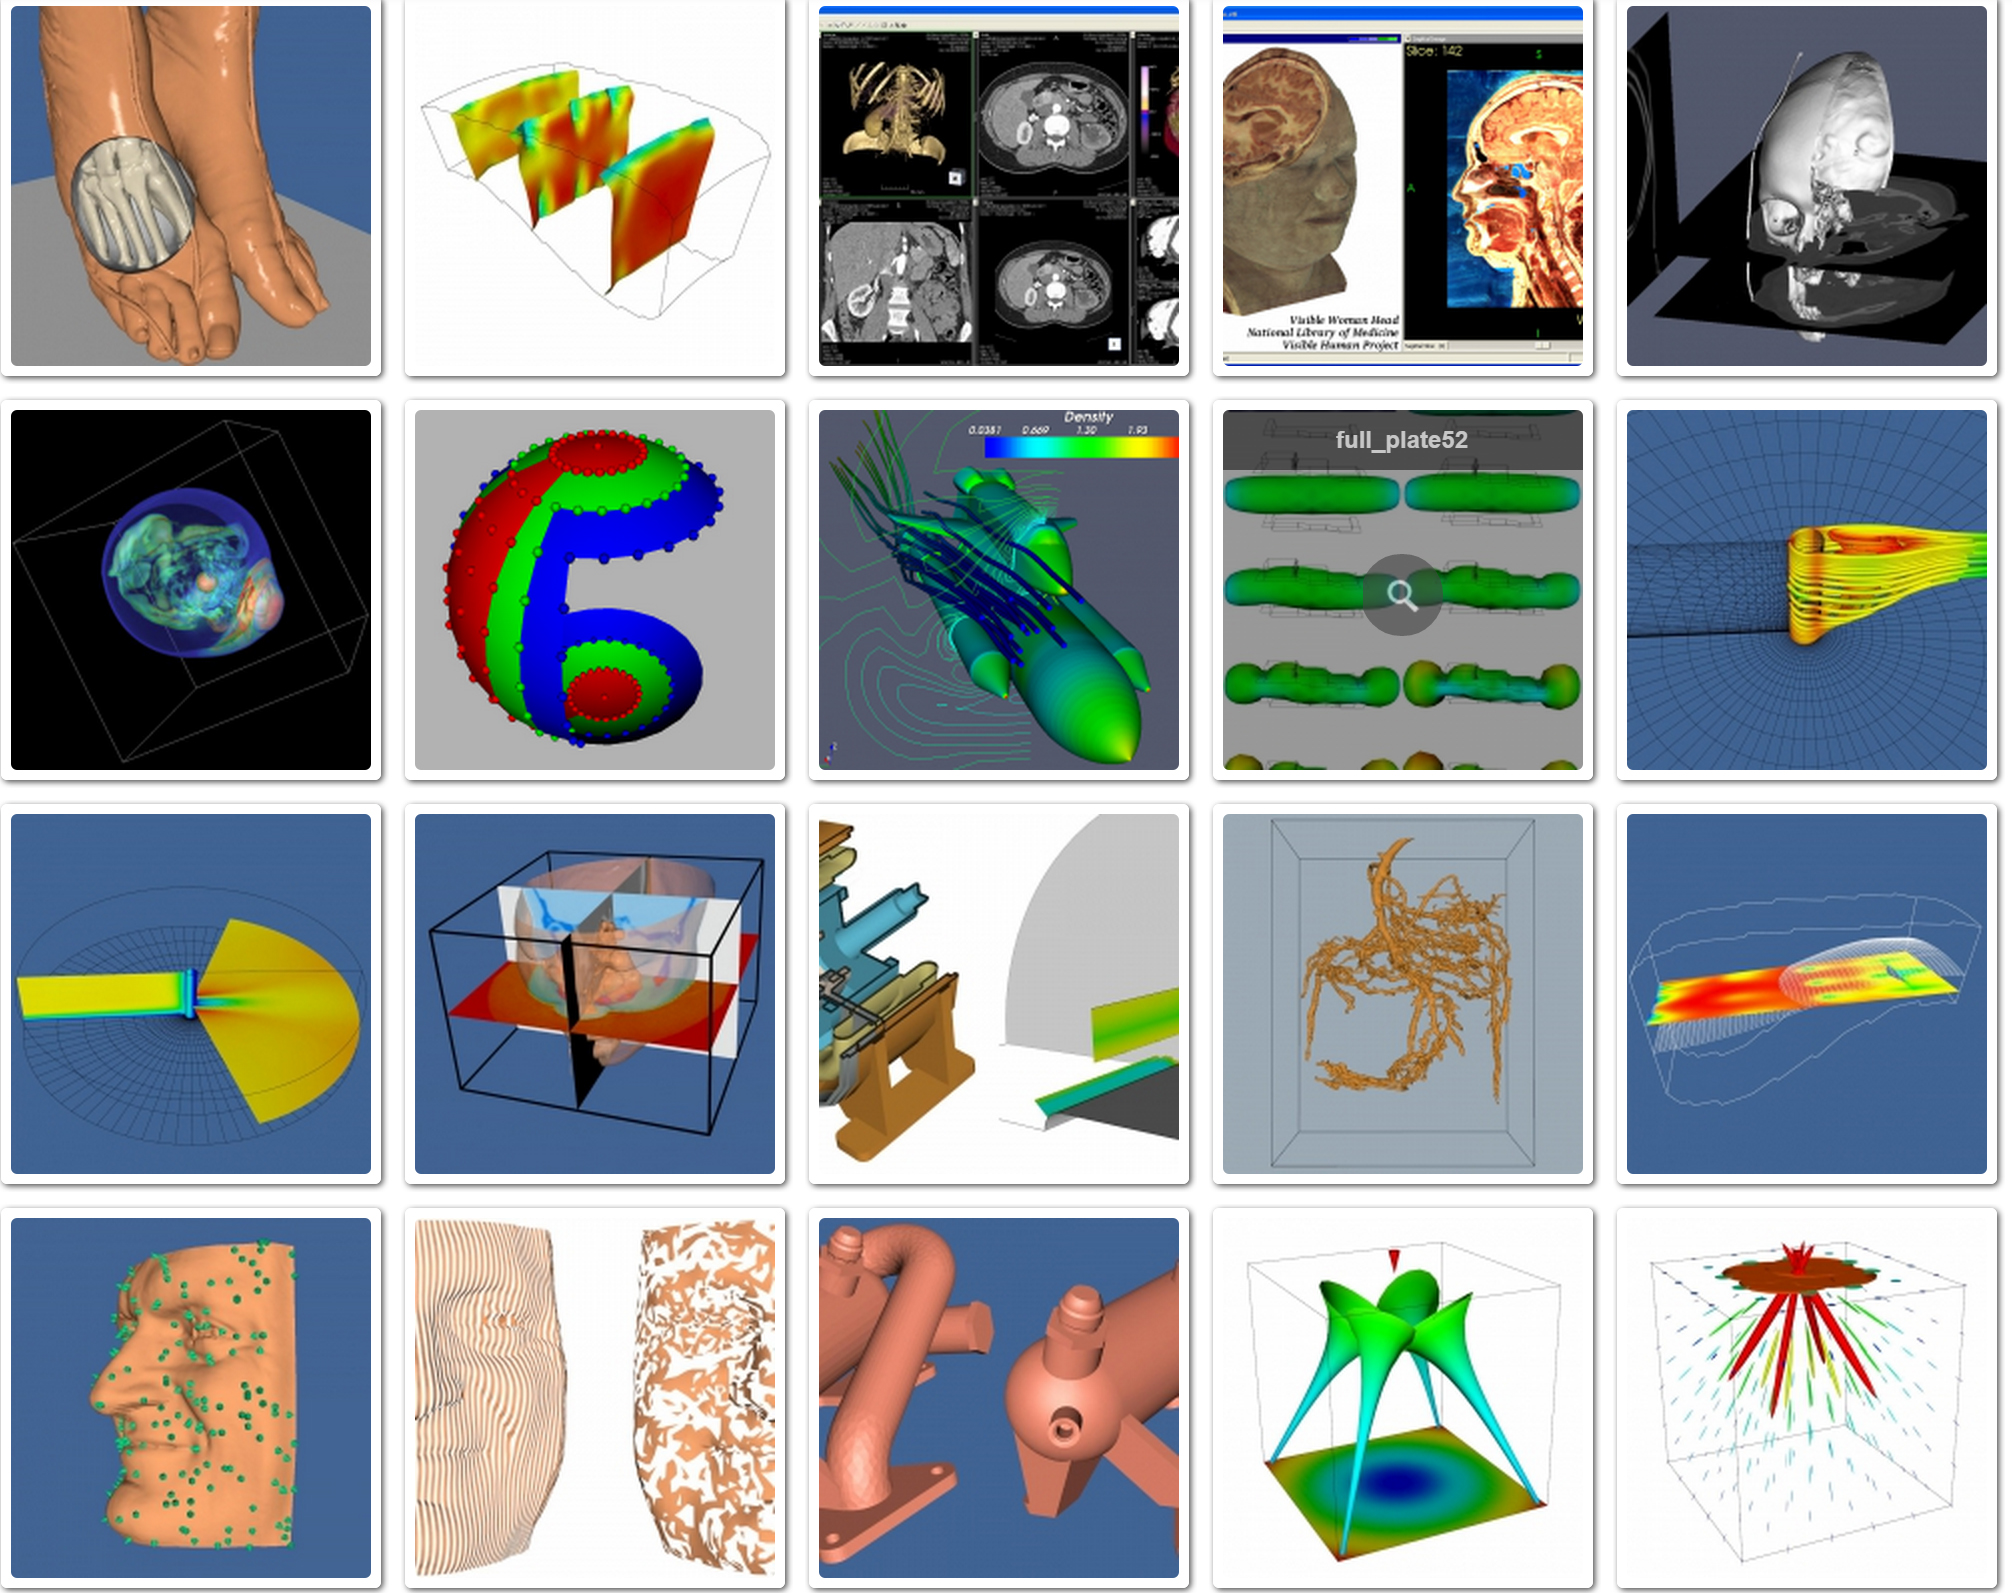
\includegraphics[width=0.9\linewidth]{graphics/vtk.jpg}
    \captionof{figure}[VTK Capabilities]{Different visualizations done with VTK.}
    \label{fig:vtkgallery}
\end{minipage}

Mayavi is probably one of the biggest open source libraries for interactive 3D visualizations in Python.
It is written almost completely in Python, but relies on \ac{VTK} for rendering.
\ac{VTK} is one of the most advanced scientific visualization library, with a huge amount of visualization types. 
In figure \ref{fig:vtkgallery} one can see some of the visualization taken from the \ac{VTK} gallery\cite{VTKGallery}.

Mayavi shares some of its goals with Romeo, namely\cite{MayaviGoals}
\begin{itemize}
	\item An (optional) rich user interface with dialogs to interact with all data and objects in the visualization.
	\item A simple and clean scripting interface in Python, including one-liners, or an object-oriented programming interface. Mayavi integrates seamlessly with Numpy and Scipy for 3D plotting and can even be used in IPython interactively, similarly to Matplotlib.
	\item The power of the VTK toolkit, harnessed through these interfaces, without forcing you to learn it.
\end{itemize}

Obviously, the Python part is not a shared goal, but creating an interactive 3D visualization library deeply embedded into a language is.
Mayavi together with VTK is a very big project and in this sense not really comparable to Romeo.
It amounts to a total of 3,642,105 lines of code written in 29 languages. The statistics can be found in table \ref{table:ParaviewStatistic} and \ref{table:VTKStatistic}.
The biggest difference is, that Romeo is implemented in a scientific programming language, while Mayavi's core uses VTK which is mainly implemented in C++.
This has two big implications.
Firstly, if the language does not have native C++ compatible data types and an overhead less C++ interface, shipping a large stream of data to VTK becomes slow.
Secondly, one must know C++ to extend VTK. This makes it difficult to create customized visualizations.

In contrast, Romeo is implemented in one language, making these tasks very simple and efficient.


\subsubsection{Vispy}

Vispy is yet another interactive 3D visualization library. It is from the goals and development status the closest to Romeo.
These include\cite{VispyGoals}:

\begin{itemize}
	\item High-quality interactive scientific plots with millions of points.
	\item Direct visualization of real-time data.
	\item Fast interactive visualization of 3D models (meshes, volume rendering).
	\item OpenGL visualization demos.
	\item Scientific GUIs with fast, scalable visualization widgets (Qt or IPython notebook with WebGL).
\end{itemize}

It is a fairly new library, promising to use modern OpenGL and being able to achieve state of the art performance.
These goals are very similar to Romeo's, with the only difference being that Romeo is completely implemented in Julia while Vispy is implemented in Python.
So the biggest differentiation between Romeo and Vispy will be found in the performance and the concrete feature set.
